\section{System}
Here, we elucidate the design and usage of each view of \textit{XGraphRAG}. 
\subsection{QA View \& Inference Trace View}

\begin{figure}[ht]
  \centering
  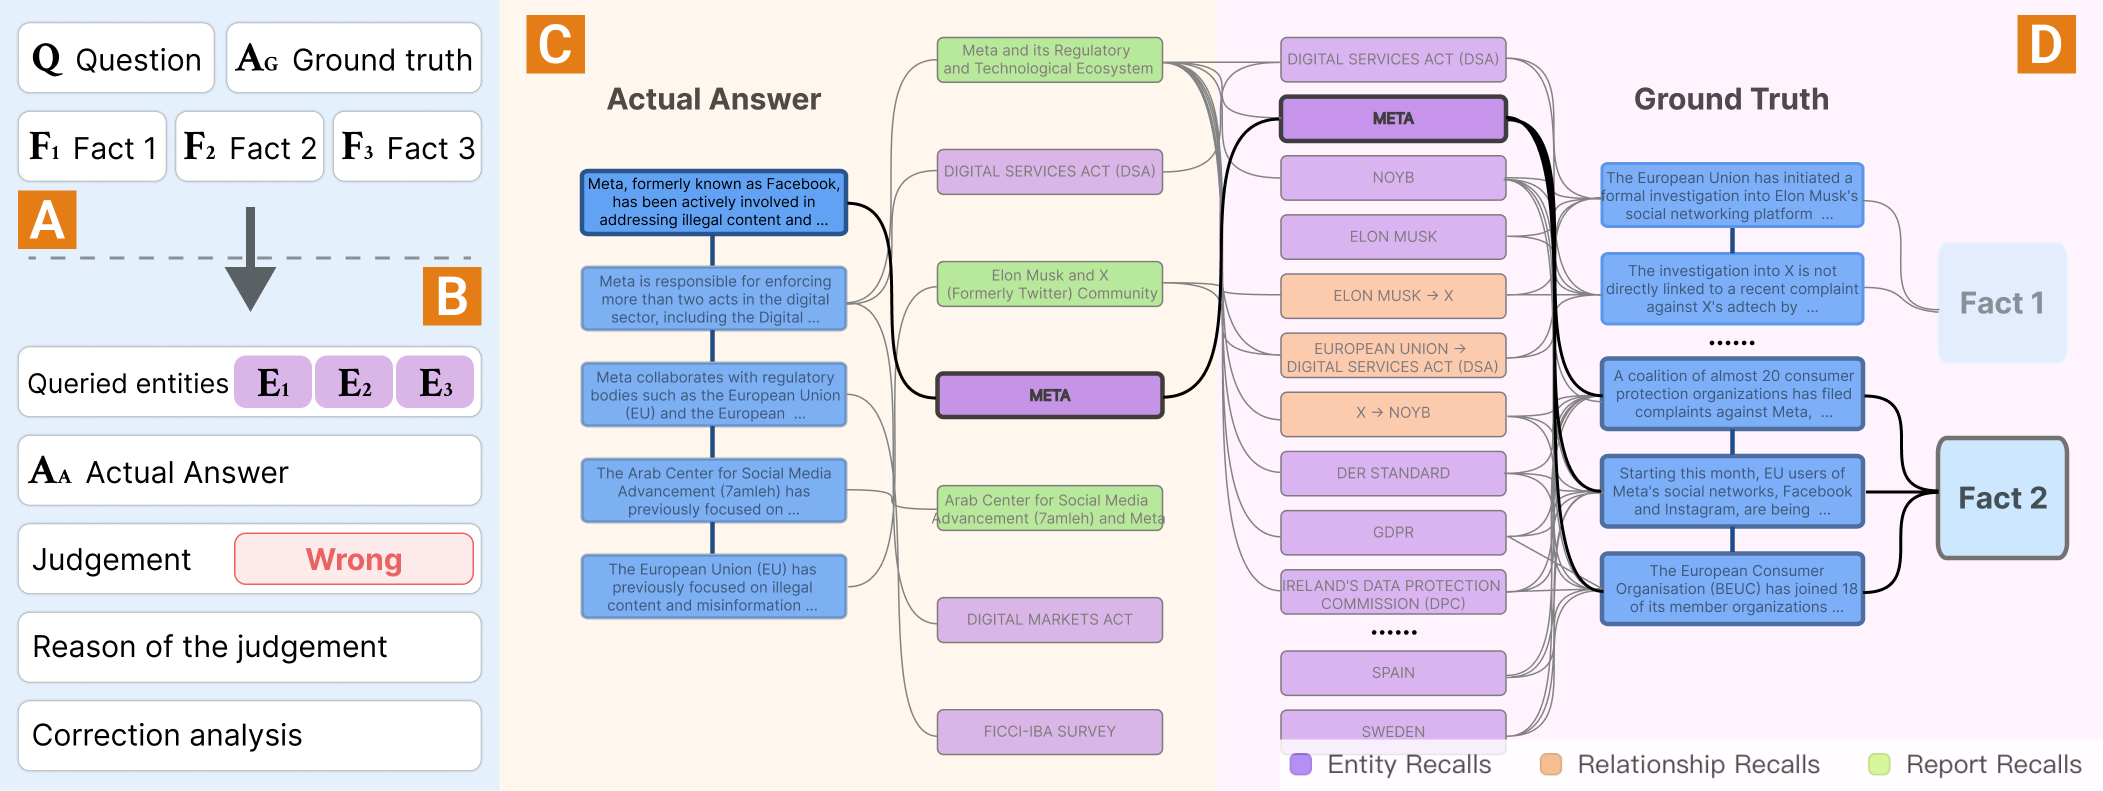
\includegraphics[width=\linewidth]{figs/QA_InferTranceView.png}
  \caption{QA View \& Inference Trace View. Once the user inputs the test question in QA View (A), the system returns key information to support discrepancy analysis (B). A detailed comparison of the
inference steps for the Actual Answer (C) and the Ground Truth (D) are shown in the Inference Trace View.}
  \label{fig:qa_infer_trace_view}
  \vspace{-10pt}
\end{figure}

The QA (Query-Answer) View (Fig~\ref{fig:qa_infer_trace_view}A) and the Inference Trace View (Fig~\ref{fig:qa_infer_trace_view}B) serve as entry points for exploration, helping users identify discrepancies between Actual Answer (Fig~\ref{fig:qa_infer_trace_view}C) and Ground Truth  (Fig~\ref{fig:qa_infer_trace_view}D). They also help users locate problematic inference steps and identify suspicious recalls (\textbf{R1}). 

\subsubsection{Analysis of Question-Answer Discrepancies}

Once users input test questions in the form $<Q, A_G, F>$ and perform queries and analyses (Fig~\ref{fig:qa_infer_trace_view}A), the system initially presents key information to support discrepancy analysis in QA View (Fig~\ref{fig:qa_infer_trace_view}B). This includes the queried entities explicitly mentioned in the question, the actual answer generated by the GraphRAG system, and the corresponding Ground Truth. Furthermore, the system provides a relevance score that evaluates the alignment between the actual answer and the Ground Truth, offering a quantitative measure of their consistency.

To further support the analysis, justifications for the relevance assessment are provided along with explanations of any observed answer discrepancies. Users can view these justifications and explanations below the Ground Truth, enabling a detailed examination of the underlying causes of discrepancies.

This initial presentation provides users with a clear and structured overview, allowing them to gain a preliminary understanding of the differences between the actual answer and the Ground Truth. It serves as a foundation for a more in-depth analysis of the reasoning and retrieval processes.

\subsubsection{Analysis of Inference Steps}

Beneath the question-answer discrepancy analysis section lies the inference step analysis section, which provides a detailed illustration of the inference steps for both the Actual Answer and the Ground Truth. This section highlights the associated query recalls for each inference step, presenting a functionally symmetric view divided into two areas.

The left section is dedicated to analyzing the inference chain of the Actual Answer (Fig~\ref{fig:qa_infer_trace_view}C). It displays the sequence of inference steps and their associated query recalls, allowing users to trace the inferring that led to the Actual Answer. The right section focuses on the Ground Truth (Fig~\ref{fig:qa_infer_trace_view}D), presenting the reference inference steps alongside their associated query recalls and the factual basis for each step.

Users can systematically compare the inference steps of the Actual Answer on the left with the inference steps of the Ground Truth on the right. This side-by-side view enables users to identify discrepancies, pinpoint problematic inference steps, and analyze the differences in the inferring stage between the two.

To further aid analysis, query recalls associated with each inference step can be traced interactively. When users hover over an inference step, the related recalls and their connections are prominently highlighted, providing immediate context for the inferring stage. In the Ground Truth section, the interface also highlights the specific facts used in each inference step, helping users quickly locate the original basis for correct reasoning. This structured approach facilitates an in-depth examination of the inferring stage and its underlying assumptions.

\subsubsection{Analysis of Recall Usage}

Users can analyze the utilization of specific query recalls within the inferring stage by interacting with the system's interface. Hovering over a query recall provides detailed information on its role in the reasoning pipeline, highlighting the following information.

First, all inference steps that involve the selected query recall are displayed, offering a clear view of how the recall contributes to the reasoning process. Second, related recalls on the opposite side, including related inferences and recalls for both the Actual Answer and the Ground Truth, are presented. For topic recalls, this includes entities or relationships encompassed within the topic recall on the opposite side. For entity-relationship recalls, identical entity or relationship recalls on the opposite side are highlighted, along with included topic recalls on the opposite side.

Additionally, related inference steps for the recalls on the opposite side are displayed, where applicable. Finally, the source of facts for the recall is revealed, whether it pertains to the Ground Truth or to related recalls on the opposite side in the Actual Answer. 

This information enables users to comprehensively analyze the query recall’s usage in the inferring stage, compare the similarities and differences between the inferring steps on both sides and efficiently identify suspicious recalls.

\subsection{Topic Explore View}

\begin{figure}[ht]
  \centering
  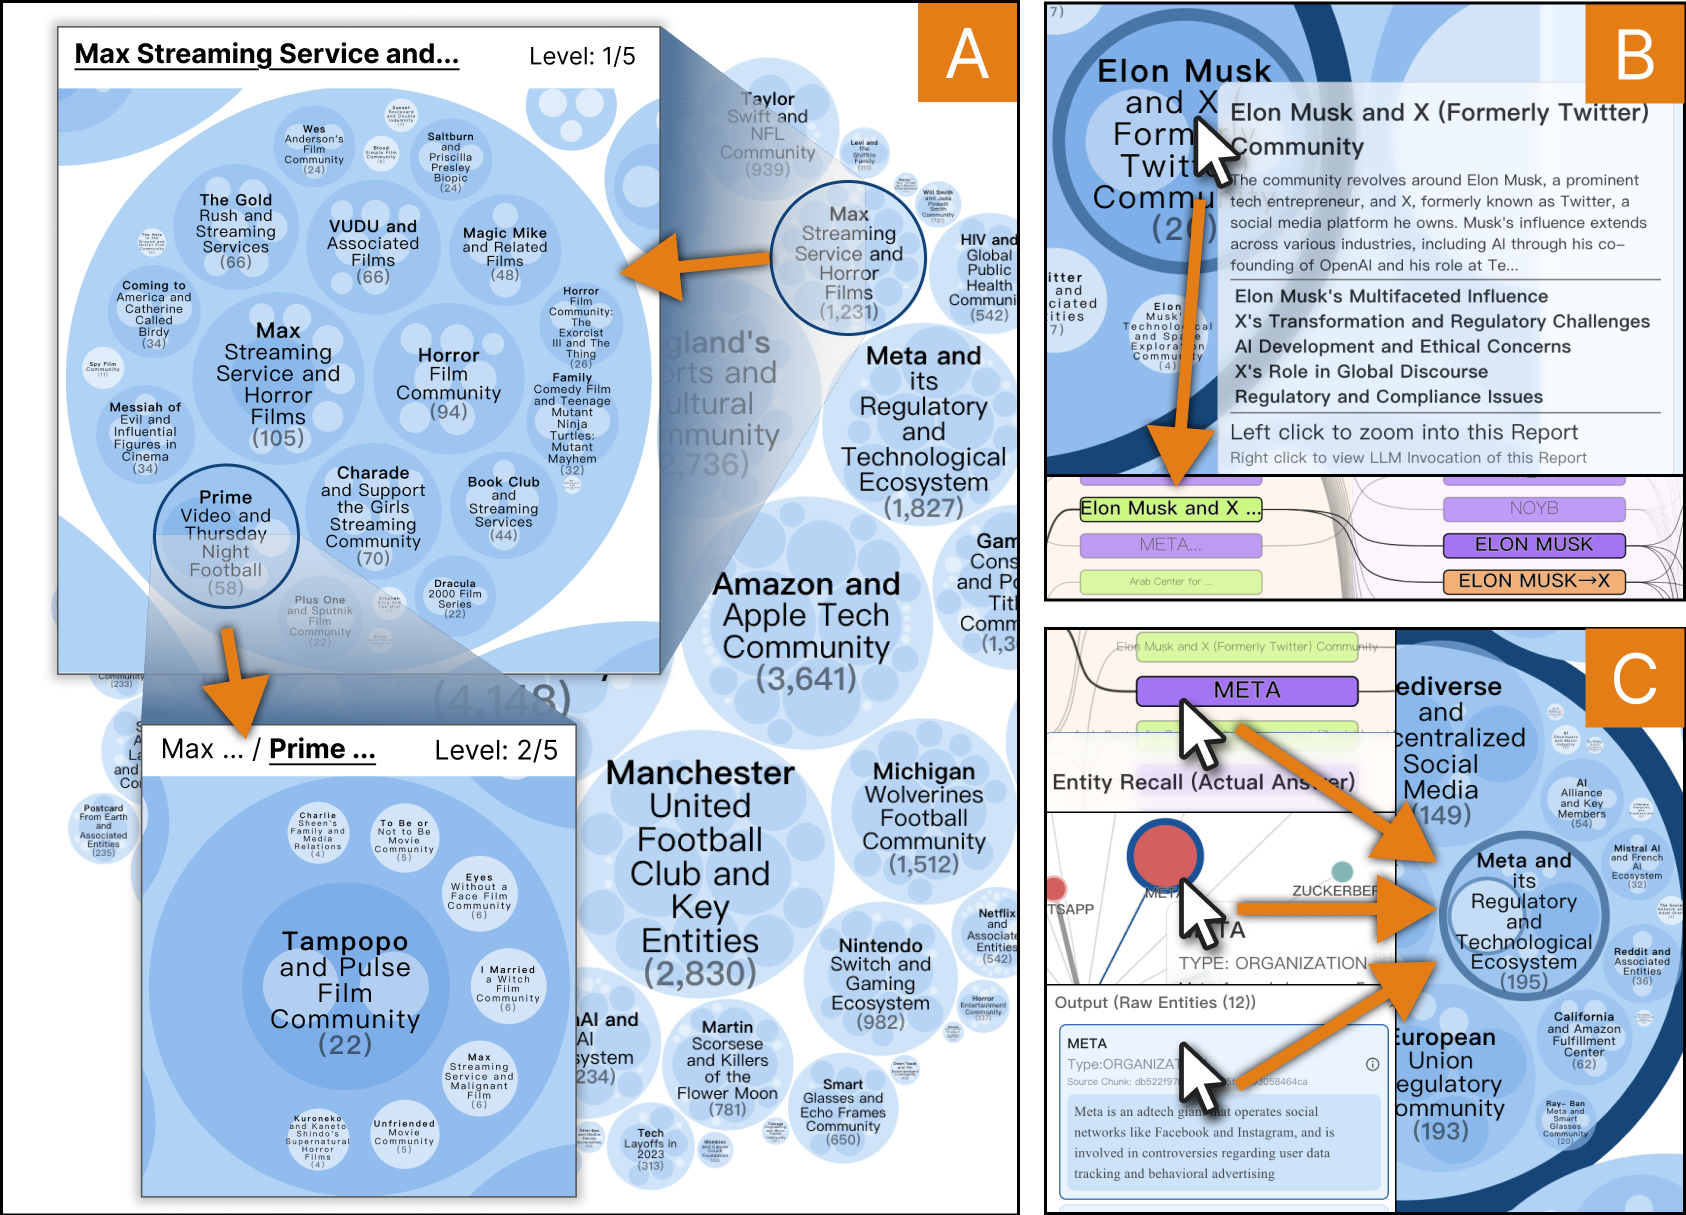
\includegraphics[width=\linewidth]{figs/TopicExploreView.png}
  \caption{Topic  Explore View, which displays all topics with explicit nesting relationships in the graph (A). Whenever the mouse hovers over a topic, the corresponding topic-type recall in the Inference Trace View will be highlighted (B). Conversely, whenever the mouse hovers over any recall in the Inference Trace View, the topic related to it will be highlighted in the Topic Explore View (C).}
  \label{fig:topic_explore_view}
\end{figure}

The Topic Explore View (Fig~\ref{fig:teaser}C) utilizes the circle packing hierarchical visualization method to display all topics with explicit nesting relationships in the graph for global relevance exploration \textbf{(R3)}. Each topic is represented by a circle at a certain level, showing the topic's title and the number of entities it contains. The number of entities is encoded as the diameter of the circle to intuitively reflect the topic's global size. Although nested circles aren't as space-efficient as treemaps, the extra space helps to better display the hierarchical structure, helping users to understand the relationships between topics more intuitively. Within each topic circle, the next-level topic circles are drawn in a lighter color, providing an intuitive understanding of the composition of subtopics. Users can click on a topic to expand and display the next-level topics it contains or explore other topics at the same level, thereby progressively exploring the composition and structure of topics in the graph (Fig~\ref{fig:topic_explore_view}A).

The Topic Explore View also provides intuitive interactions to help trace the relationship between a topic and its related recalls: As shown in (Fig~\ref{fig:topic_explore_view}B), whenever the mouse hovers over a topic, the corresponding topic-type recall in the Inference Trace View will be highlighted. Conversely, as shown in Fig~\ref{fig:topic_explore_view}C), whenever the mouse hovers over any recall in the Inference Trace View, the topic related to it will be highlighted in the Topic Explore View. This facilitates quick exploration of global semantic relationships among different entities, relationships, and topics.


% Whenever users identify a suspicious recall in the Inference Trace View, they can hovers over it to further examine it in 


% the Topic exploration view can assist in examining its positioning within the system: when the mouse hovers over a topic-type recall in the Inference Trace View, the Topic exploration view emphasizes the topic and all its upper-level topics (Fig~\ref{fig:topic_explore_view}B); when the mouse hovers over an entity or relationship-type recall in the Inference Trace View, the Global exploration view emphasizes all topics containing the entity or relationship (Fig~\ref{fig:topic_explore_view}C). This facilitates quick exploration of global semantic relationships among different entities, relationships, and topics.

\subsection{Entity Explore View}

\begin{figure}[ht]
  \centering
  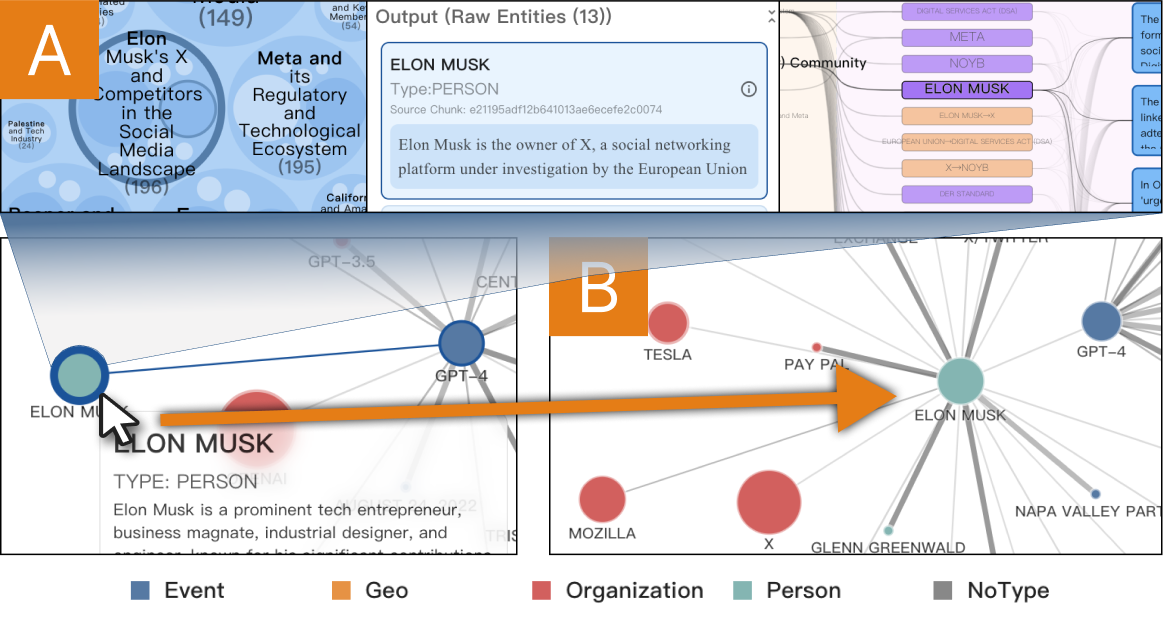
\includegraphics[width=\linewidth]{figs/EntityExploreView.png}
  \caption{The Entity Explore View enables investigation of entity recalls through a node-link diagram. Node size encodes entity frequency, edge thickness shows topic distance, and node color indicates entity type. Interactive highlighting helps trace elements across different views (A). Users can expand the local graph by right-clicking nodes/edges to explore related entities and relationships (B).}
  \label{fig:entity_explore_view}
  \vspace{-10pt}
  
\end{figure}

The Entity Explore View (Fig~\ref{fig:teaser}D) assists users in investigating the local relevance of suspicious entity recalls with other entity recalls and relationship recalls \textbf{(R4)}. Whenever users identify a suspicious entity recall in the Inference Trace View, they can right-click to add it to the list in the Entity Explore View. Subsequently, users can utilize this view to explore other entities and relationships associated with the identified entity. We use a node-link diagram to visualize the local subgraph around this entity. Here the diameter of each node encodes the number of times it appears in different text chunks, intuitively reflecting the frequency and importance of the entity. The thickness of the edge encodes the distance of nodes in the nested topic tree, which also determines the strength of attraction in the force-directed layout. The node color encodes the types of entities. To ensure that each type has a distinctly different yet soft color, we use the HSL model, evenly sampling the hue values while maintaining moderate saturation and lightness. To help users better trace entities and relationships across views, whenever they hover over an entity point or relationship edge in the local graph, it will also be highlighted in other views (Fig~\ref{fig:entity_explore_view}A). If the user wants to explore more about a certain node/edge, they can right-click on it to add more entities and relationships near it (Fig~\ref{fig:entity_explore_view}B).


% related entities and relationships are highlighted. Furthermore, when the mouse hovers over an entity point, if the entity appears as a recall in the Inference Trace View, the recall and usage links are prominently displayed, and all topics containing the entity are highlighted in the Global exploration view (Fig~\ref{fig:entity_explore_view}A). If users wish to continue exploring relevance based on a point, they can right-click on it, and the local graph will add entities and relationships related to the point (Fig~\ref{fig:entity_explore_view}B).

\subsection{LLM Invocation View}

\begin{figure}[ht]
  \centering
  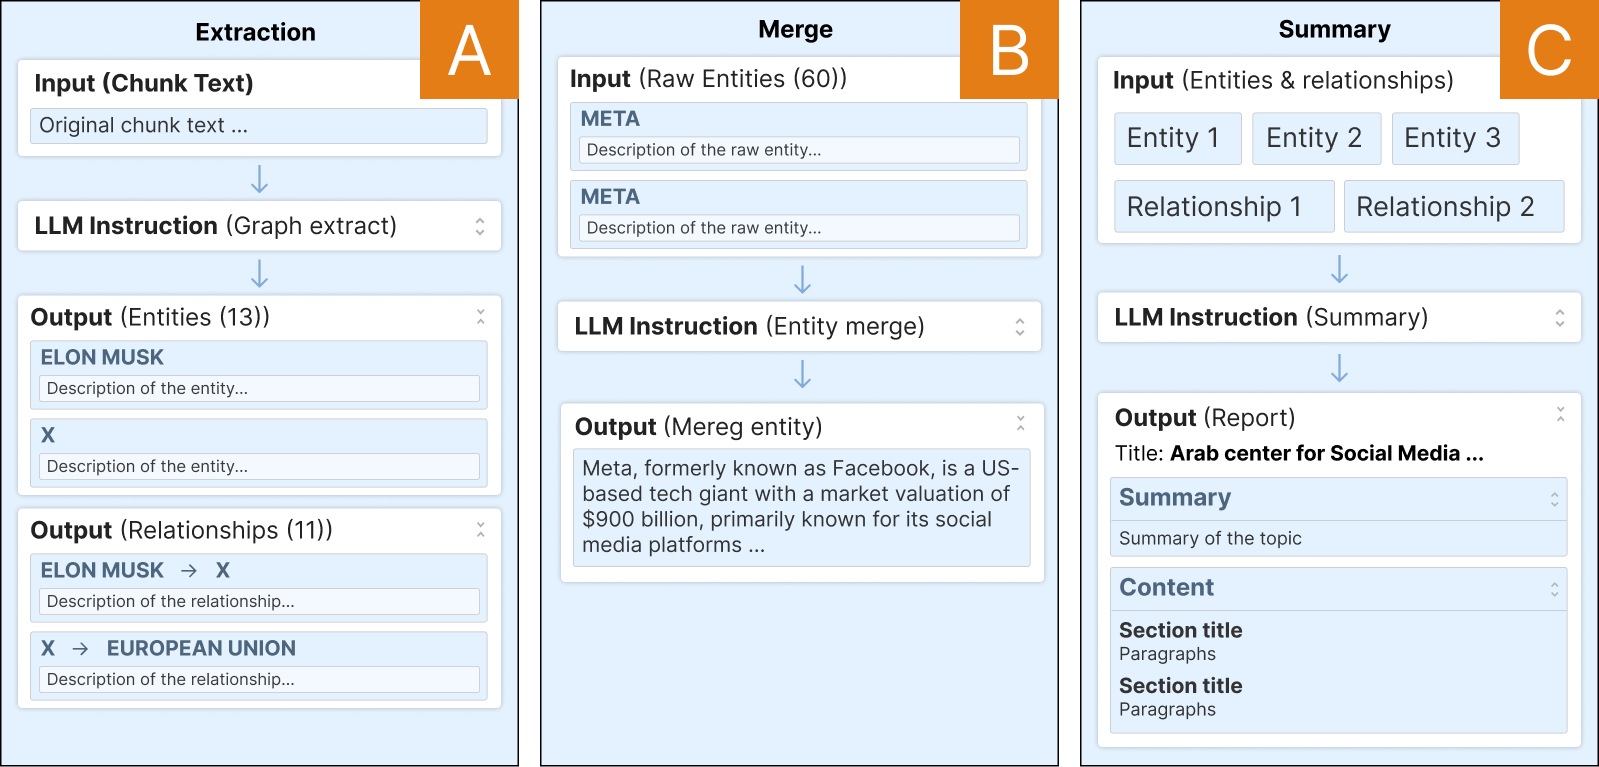
\includegraphics[width=\linewidth]{figs/LLMIvocationView.png}
  \caption{The LLM Invocation View has three variations, showing LLM behaviors during different stages of graph construction: extraction stage view displays source chunks and extraction details (A), merge stage view presents entity/relationship integration process (B), summary stage view reveals topic report generation with related entities and relationships (C).}
  \label{fig:llm_invocation_view}
  \vspace{-10pt}
\end{figure}

The LLM Invocation View (Fig~\ref{fig:teaser}E) reveals the behaviors of the LLM during various stages of graph construction in the GraphRAG system \textbf{(R2)}. This view has three variations for different stages, as elaborated below.

\subsubsection{Summary Stage LLM Analysis}

Whenever users click on any topic recall in any view, the related information of the topic and the behavioral details of the LLM in generating the topic report during the summary stage are displayed in the LLM Invocation View (see Fig~\ref{fig:llm_invocation_view}C). Users can investigate the entities and relationships used by the LLM in the summary process, the structure of the LLM's prompt words, and the topic report generated by the LLM. Since many entities and relationships may be used in topic summaries, this part can also link with other views for related information highlighting and filtering. For example, when the mouse hovers over an entity-relationship recall or fact in the Inference Trace View, or an entity point or relationship edge in the Entity Explore View, related entities and relationships are highlighted at the top of the list. This allows for quick confirmation of whether there is a relevant link between the part of the graph used for the topic and the object to be explored.

\subsubsection{Merge Stage LLM Analysis}

Whenever users click on any entity or relationship recall in any view, the related information of the entity/relationship and the behavior details of the LLM in processing the entity or relationship during the merge stage are displayed in the LLM
Invocation View (see Fig~\ref{fig:llm_invocation_view}B). Users can investigate the original entities or relationships used by the LLM in the merge process, the structure of the LLM's prompt words, and the merge results generated by the LLM. This information helps users understand how the LLM processes and integrates entity or relationship information from different sources and further traces the source of information for entities or relationships. Similarly, this view links with other views for hover-highlighting, enabling fluid tracing.

\subsubsection{Extraction Stage LLM Analysis}

Whenever users click on any fact or any entity or relationship during Merge Stage LLM Analysis, the source chunk information of the original entity or relationship and the behavior details of the LLM in the extraction stage are displayed in the LLM
Invocation View (see Fig~\ref{fig:llm_invocation_view}A). Then users can delve into how the LLM extracts entities and relationships from the original text using this information. This transparency helps users evaluate the reliability and accuracy of the information while also laying the foundation for further data quality improvement. Additionally, this view can help users trace the source of specific information, thereby better understanding and verifying the system's inference process.